\documentclass{article}
\usepackage[margin=1in]{geometry}
\usepackage[nodisplayskipstretch]{setspace}
\usepackage{amsmath, nccmath, bm}
\usepackage{amssymb}
\usepackage{enumitem}
\usepackage{graphicx}
\usepackage{float}
\usepackage{listings}
\usepackage{hyperref}
\usepackage[svgnames]{xcolor}
\usepackage{indentfirst}
%\usepackage{chngcntr}
%\counterwithin{table}{section}
\graphicspath{
{./images}}

%\hypersetup{
%    colorlinks=true,
%    linkcolor=black,
%    filecolor=black,      
%    urlcolor=blue
%    }

\newcommand{\zerodisplayskip}{
	\setlength{\abovedisplayskip}{0pt}%
	\setlength{\belowdisplayskip}{0pt}%
	\setlength{\abovedisplayshortskip}{0pt}%
	\setlength{\belowdisplayshortskip}{0pt}%
	\setlength{\mathindent}{0pt}}
	
\definecolor{vgreen}{RGB}{104,180,104}
\definecolor{vblue}{RGB}{49,49,255}
\definecolor{vorange}{RGB}{255,143,102}

\lstdefinestyle{verilog-style}
{
    language=Verilog,
    basicstyle=\small\ttfamily,
    keywordstyle=\color{vblue},
    identifierstyle=\color{black},
    commentstyle=\color{vgreen},
    numbers=left,
    numberstyle=\tiny\color{black},
    numbersep=10pt,
    tabsize=8,
    moredelim=*[s][\colorIndex]{[}{]},
    literate=*{:}{:}1
}

\lstset{style={verilog-style},showstringspaces=false}

\lstdefinestyle{nocoloring}{
    keywordstyle=\color{black},
    commentstyle=\color{black},
    stringstyle=\color{black}
}

\makeatletter
\newcommand*\@lbracket{[}
\newcommand*\@rbracket{]}
\newcommand*\@colon{:}
\newcommand*\colorIndex{%
    \edef\@temp{\the\lst@token}%
    \ifx\@temp\@lbracket \color{black}%
    \else\ifx\@temp\@rbracket \color{black}%
    \else\ifx\@temp\@colon \color{black}%
    \else \color{vorange}%
    \fi\fi\fi
}
\makeatother

\newcommand{\code}[1]{%
	\colorbox{Gainsboro}{\texttt{#1}}%
}

\title{Lab 2}
\author{Owen Sowatzke}
\date{March 31, 2025}

\begin{document}

	% \offinterlineskip
	% \setlength{\lineskip}{12pt}
	% \zerodisplayskip
	\maketitle
	
	\section{Introduction}
	
	\section{NAND Gate}
	
	\subsection{Layout}
	
	\begin{figure}[H]
		\centerline{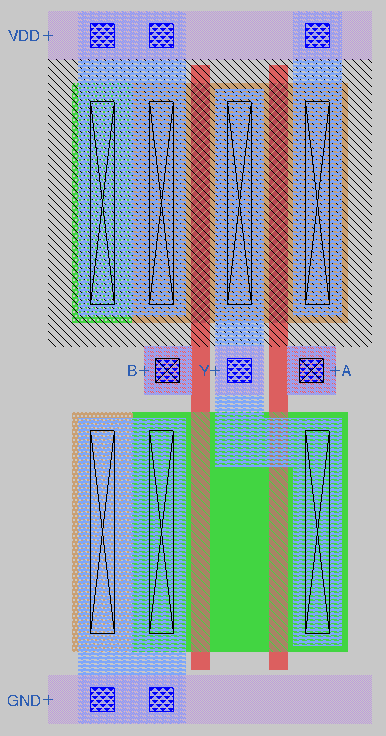
\includegraphics[width=0.3\textwidth]{nand_layout.png}}
		\caption{NAND Layout}
		\label{fig::nand_layout}
	\end{figure}

	\begin{figure}[H]
		\centerline{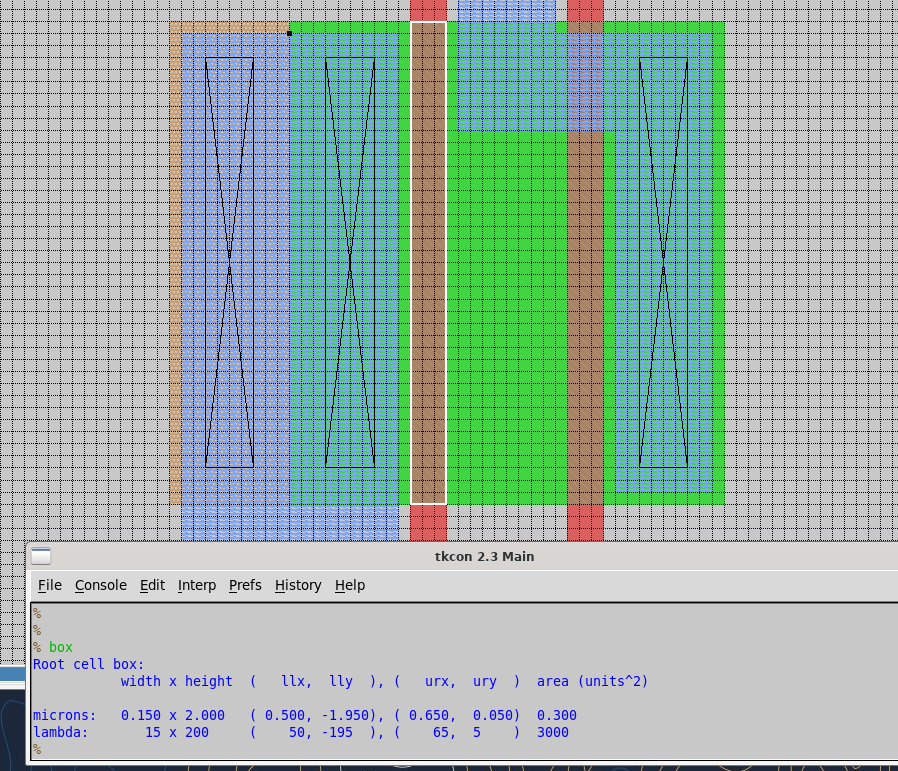
\includegraphics[width=0.5\textwidth]{nand_nmos_channel_sizing.png}}
		\caption{Checking NMOS Channel Size}
		\label{fig::nand_nmos_channel_sizing}
	\end{figure}
	
	\begin{figure}[H]
		\centerline{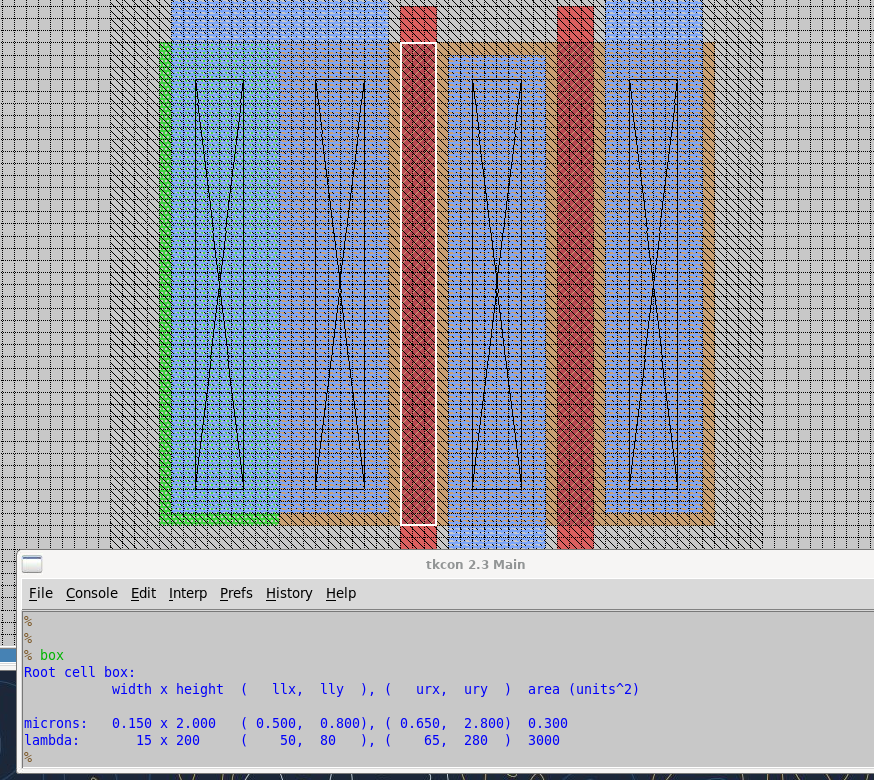
\includegraphics[width=0.5\textwidth]{nand_pmos_channel_sizing.png}}
		\caption{Checking PMOS Channel Size}
		\label{fig::nand_pmos_channel_sizing}
	\end{figure}
	
	\begin{figure}[H]
		\centerline{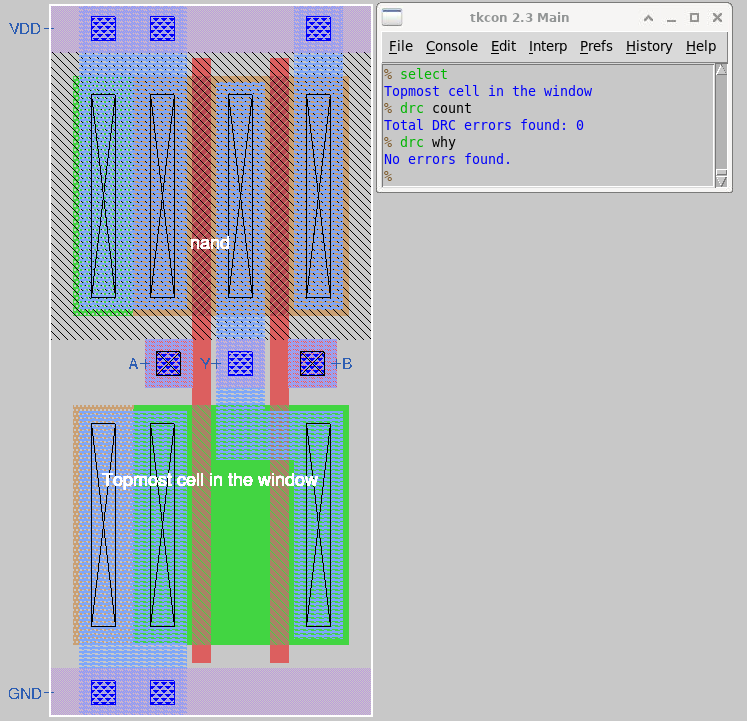
\includegraphics[width=0.5\textwidth]{nand_drc_errors_terminal.png}}
		\caption{Checking DRC Errors from Terminal}
		\label{fig::nand_drc_errors_terminal}
	\end{figure}
	
	\begin{figure}[H]
		\centerline{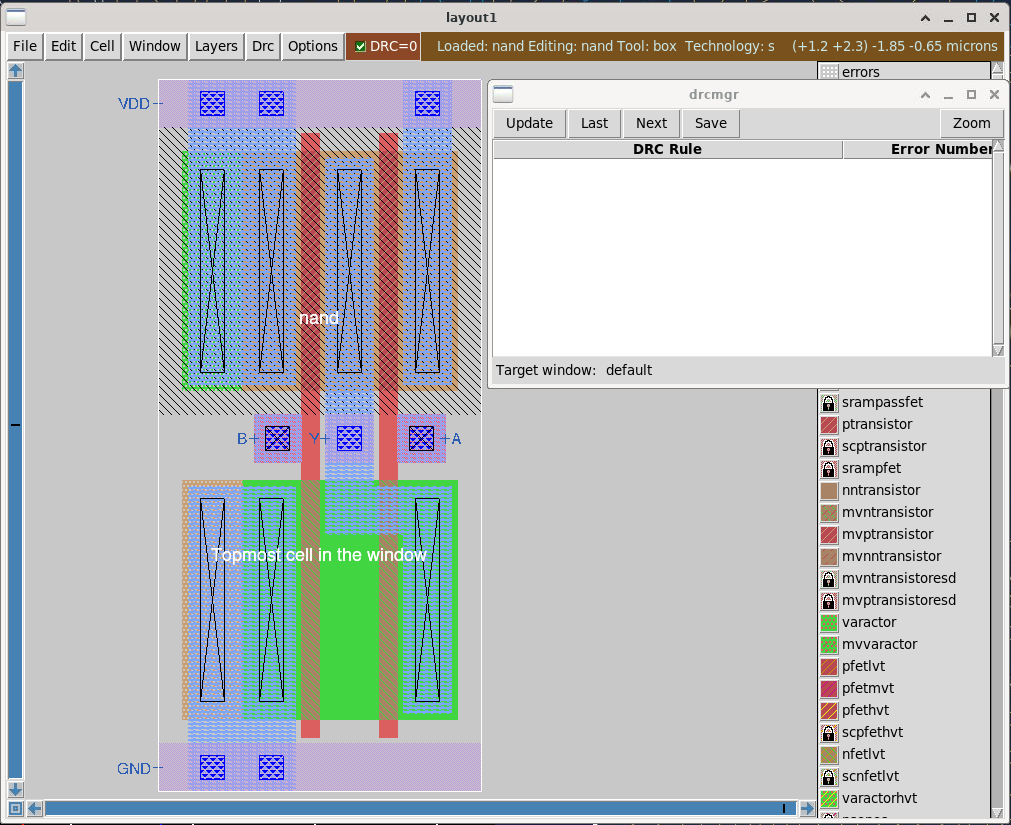
\includegraphics[width=0.5\textwidth]{nand_drc_errors_drcmgr.png}}
		\caption{Checking DRC Errors with drcmgr}
		\label{fig::nand_drc_errors_drcmgr}
	\end{figure}
	
	\subsection{Netlist}
	
	\begin{figure}[H]
		\centerline{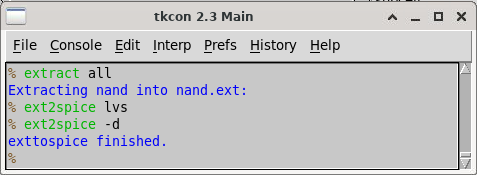
\includegraphics[width=0.3\textwidth]{nand_netlist_creation.png}}
		\caption{SPICE Netlist Extraction}
		\label{fig::nand_netlist_creation}
	\end{figure}
	
	\begin{figure}[H]
		\lstinputlisting[style=nocoloring,frame=single]{./src/nand.spice}
		\caption{Extracted SPICE Netlist}
		\label{fig::nand_netlist}
	\end{figure}
	
	\begin{figure}[H]
		\lstinputlisting[style=nocoloring,frame=single,basicstyle=\fontsize{7}{7}\selectfont\ttfamily]{./src/nand_vtc.spice}
		\caption{Test Circuit to Extract VTC from Netlist}
		\label{fig::nand_vtc_extraction}
	\end{figure}
\end{document}